\chapter{Lösungsansatz}\label{chp:loesungsansatz}

Um  den Lösungsansatz besser zu verstehen, wird erst der Ablauf von der Erstellung der Anforderung bis zu einem Testfall erläutert. Zuerst werden in DOORS alle schon vordefinierten Anforderungen eingetragen (siehe \ref{sec:DOORS}). In diesen Anforderungen können Parameter vorkommen, die für die Testfälle relevant sind. Die Parameter werden folgendermaßen in einer Anforderung eintragen:\\

\begin{center}
\#param [\textit{Parametername}]\\
\#param [max\_Geschwindigkeit]\\
Das Auto hat eine Maximalgeschwindigkeit von \#param[max\_geschwindigkeit] km/h
\end{center}

Die Parameter sind in einer Parameter-Tabelle definiert, in der die jeweiligen Parameterwerte eingetragen werden. Der Grund, warum es eine gesonderte Tabelle für Parameter gibt, kommt daher, dass die Parameter in der Regel pro Variante verschiedene Werte annehmen. Zum Beispiel beträgt die maximale Geschwindigkeit bei einem Cabrio 100 km/h  und bei einem Kombi 150 km/h. Dank dieser Tabelle werden den Varianten (Cabrio und Kombi) die richtige Parameterwerte zugewiesen.\\


Da Parameterwerte und Varianten schon verlinkt sind, müssen die Anforderungen, die Parameter beinhalten, mit der Parametertabelle manuell verlinkt werden. Wenn dieser Vorgang abgeschlossen ist, kann über die TESTONA Oberfläche die Verbindung zu DOORS aufgebaut werden um die nötigen Informationen zu importieren. Voraussetzung ist, dass der Tester bereits einen Klassifikationsbaum passend zum zu testenden Produkt und die dazu gehörige Anforderungen erstellt hat. Jetzt können die in DOORS definierten Varianten importiert werden. Zunächst muss der Tester die Baumelemente der richtigen Variante zuordnen (durch ein Ausschlussverfahren wird angenommen, dass alle Baumelemente in allen Varianten gültig sind). 


%#######################################################################################
%#######################################################################################
\newpage
\section{Parameterspeicherung}\label{sec.parameterspeicherung}
\paragraph{}
 
Um die Parameter erfolgreich in TESTONA zu speichern, müssen diese aus DOORS importiert werden und aus den Anforderungen gelesen werden. Durch eine gezielte Anfrage an DOORS, über eine Java API, kann die Parametertabelle in TESTONA geladen werden. Die darin bestimmten Beziehungen (Parameterwert zu Variante) müssen fest in die TESTONA Datei gespeichert werden, damit diese auch ohne eine DOORS Verbindung zur Verfügung steht. Als erstes werden die Parameterwerte in \textit{Tag} Objekten gespeichert und nach Programmende in die TESTONA Datei im XML Format gespeichert. Dank des \textit{Tags} kann beim Programmstart wieder der Parameterwert gelesen werden und während das Programm ausgeführt wird können Änderungen vorgenommen werden.\\


Einer der Besonderheiten von TESTONA ist, dass Anforderungen und Baumelemente per Drag\&Drop verknüpft werden können. Mit dieser Funktion muss der Tester die Anforderung mit einem dazu gehörigen Baumelement verknüpfen (auslösendes Ereignis der Parameterspeicherung). Damit das Programm die Aktion des Benutzers mitbekommt, wird an dieser Stelle ein \textit{Listener} implementiert. Der \textit{Listener} bekommt verschiedene Nachrichten von Ereignissen die gefiltert werden müssen. Wenn die Nachricht empfangen wird, dass eine Anforderung an ein Baumelement verknüpft wurde, muss eine zu programmierende Methode den Anforderungstext von diesem Baumelement lesen und nach Parametern suchen. Als erstes wird davon ausgegangen, dass ein Baumelement nur eine Anforderung beinhalten kann und eine Anforderung nur ein Parameter beinhaltet. Wird in der gelesenen Anforderung ein Parameter gefunden, so müssen die möglichen Werte dieses Parameters aus der DOORS Parametertabelle gelesen und gespeichert werden. An dieser Stelle beginnt die Parameterspeicherung.\\


Für die Parameterspeicherung ergeben sich zwei Lösungswege. Die erste Lösung lautet, die Parametertabelle beim Import der Anforderung gleich in TESTONA zu speichern. Diese Lösung hat den Vorteil, dass später eine Verbindung zu DOORS nicht mehr notwendig ist. Somit muss während der Parametersuche auf eine Verbindung mit DOORS nicht geprüft werden, bzw. die Verbindung muss nicht wieder aufgebaut werden. Das heißt der Benutzer muss sich nur einmal mit DOORS verbinden und kann in der Zukunft problemlos die Anforderungen an einem Baumelement verlinken und gleichzeitig werden die Parameter gelesen und gespeichert. Der Nachteil ist, dass möglicherweise unnötige Daten in TESTONA gespeichert werden.\\


Die zweite Lösung ist gegensätzlich zu der ersten Lösung. Hier werden jeweils nur die Daten gespeichert, die der Benutzer im Moment benötigt. Wird eine Anforderung an einem Baumelement verlinkt, so muss eine Verbindung zu DOORS aufgebaut werden und die Parametertabelle aufgerufen und in TESTONA gespeichert werden. Der große Nachteil dieser Lösung ist, dass der Benutzer möglicherweise keine Verbindung zu DOORS aufbauen kann. Zum Beispiel, wenn der Server nicht vorhanden ist, keine Zugriffsmöglichkeiten, etc. Welcher der beiden Lösungen implementiert wird, wird erst noch genauer analysiert. Die Lösung ist auch abhängig von den Anforderungen verschiedener Kunden und wie diese TESTONA anwenden. Die implementierte Lösung wird in Kapitel \ref{chp:systementwurf} vorgestellt und begründet.\\


Sind die Parameterwerte in TESTONA vorhanden, müssen diese der richtigen Variante zugeordnet werden. Dafür ist vorgesehen, dass der Parameterwert als Eigenschaft des Baumelementes gespeichert wird (als ein \textit{Tag} Objekt). Die Darstellungsstruktur für die Variantenansicht ist folgendermaßen definiert:\\

\begin{figure}[h!]
  \begin{center}
    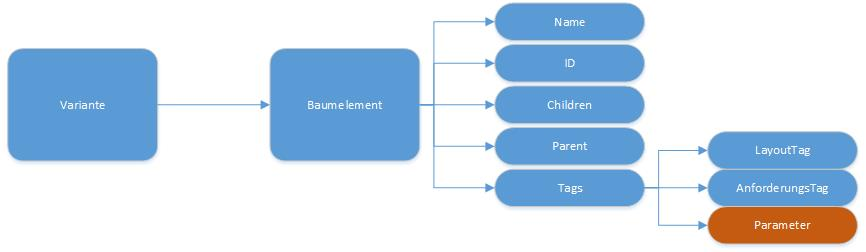
\includegraphics[scale=0.65]{4_1_UML_Var_TreeItem_Properties.jpg}
  		  \caption{Darstellung der TESTONA Objekte für die Parameterspeicherung}
     \label{ttn.objectGraph}
  \end{center}
\end{figure}

\hspace{2cm}

Somit kann jetzt in TESTONA ein Parameterwert mit einer Variante und einem Baumelement verknüpft werden. Als Ergebnis werden folgenden Beziehungen erwartet:

\begin{center}
\textbf{Anforderung 1: }Das Auto hat eine Maximalgeschwindigkeit von \#param[max\_Geschwindigkeit] km/h.
\end{center}

\begin{table}[h]
\begin{center}
	\begin{tabular}{|l||c|c|}
	 \hline
	 Variante &max\_Geschwindigkeit &Anforderung\\
	 \hline\hline
	 Cabrio   &100                      & 1\\
	 \hline
	 Kombi    &150                      & 1\\
	 \hline
	 Limo     &250                      & 1\\
	 \hline
	\end{tabular}
	
	\caption{Beispiel für die Zuordnung zwischen Varianten und Parameterwert aus einer Anforderung}
	\label{table:Zuordnung}
\end{center}
\end{table}

Wichtig ist auch, dass ein Baumelement verschiedene Parameter repräsentieren kann. Wenn ein Baumelement mehr als eine Anforderung mit verschiedenen Parametern beinhaltet, wird die aktive Variante entscheiden, welches Parameter ausgewertet  und angezeigt wird. Dabei muss beachtet werden, dass vorhandene Parameterwerte und Anforderung (innerhalb eines Baumelementes) nicht gelöscht oder überschrieben werden.\\

\begin{figure}[h!]
  \begin{center}
    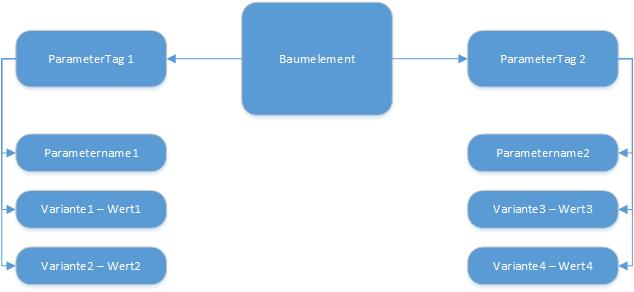
\includegraphics[scale=0.7]{4_1_UML_TreeItem_ParameterTags.jpg}
  		  \caption{Darstellung eines Baumelementes mit zwei verschiedene Parametern und vier Varianten}
     \label{ttn.treeitem_vars}
  \end{center}
\end{figure}

%#######################################################################################
%#######################################################################################
\newpage
\section{Visualisierung}\label{sec.visualisierung}
\paragraph{}

Wenn die Beziehungen zwischen Varianten, Parametern und Anforderungen erfolgreich entstanden sind, können jetzt die gespeicherten Parameterwerte angezeigt werden. Wenn der Benutzer die Varianatenansicht in der Benutzeroberfläche ändert, die Beschriftung (\textit{Label}) des Bauelementes (Maximalgeschwindigkeit von Generic = X, Cabrio = 150, Kombi = 200) muss eine Aktualisierung erfolgen.


\begin{figure}[h!]
  \begin{center}
    
\includegraphics{4_2_Change_Var_Generic.png}
    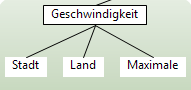
\includegraphics[scale=0.8]{4_2_Change_Var_Generic_Tree.png}
  		  \caption{Aktive Variante Generic (default)}
     \label{ttn.generic}
  \end{center}
\end{figure}

\begin{figure}[h!]
  \begin{center}
    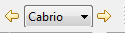
\includegraphics{4_2_Change_Var_Cabrio.png}
    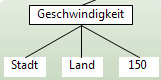
\includegraphics[scale=0.9]{4_2_Change_Var_Cabrio_Tree.png}
  		  \caption{Aktive Variante Cabrio}
     \label{ttn.2}
  \end{center}
\end{figure}

\begin{figure}[h!]
  \begin{center}
    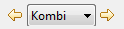
\includegraphics{4_2_Change_Var_Kombi.png}
    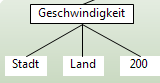
\includegraphics[scale=0.9]{4_2_Change_Var_Kombi_Tree.png}
  		  \caption{Aktive Variante Kombi}
     \label{ttn.3}
  \end{center}
\end{figure}

Dafür muss ein \textit{Listener} beim Ändern der Variantenansicht eine Methode aufrufen. Diese aktualisiert die Werte und die Neuzeichnung der Baumelemente. Die Werten werden dynamisch aus den Inhalten der Baumelemente gelesen. Zur Erinnerung: Die Werte sind als \textit{Tag} im jeden Baumelement gespeichert (siehe Abbildungen \ref{ttn.objectGraph} und \ref{ttn.treeitem_vars}).


%#######################################################################################
%#######################################################################################
\newpage
\section{Testgültigkeit}
\paragraph{}
%Innerhalb einer Variante auf Testfallduplikate überprüfen anhand der Paramerterwerte
%Testfallabdeckung + Prozessoptmierung
Wenn TESTONA in der Lage ist, die Parameterwerte abhängig von der Variante darzustellen, soll möglicherweise nach duplizierten Testfällen gesucht werden. Es kann dazu kommen, dass sich ein Testfall dupliziert, da zwei oder mehrere Parameter den gleichen Wert besitzen. Ein einfaches Beispiel:\\

\begin{figure}[h!]
  \begin{center}
    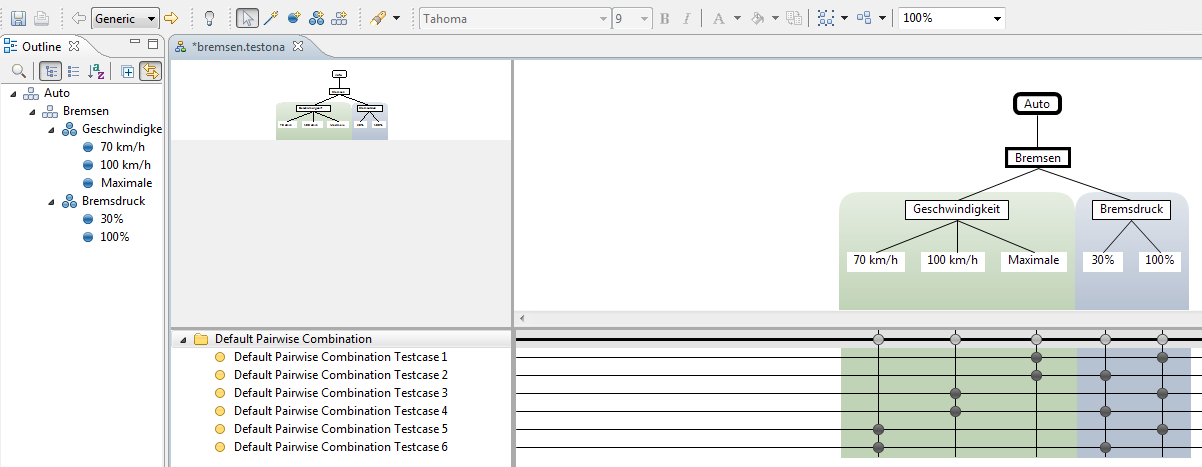
\includegraphics[scale=0.4]{4_3_generic.png}
  		  \caption{Das generische Baum}
     \label{ttn.cases_generic}
  \end{center}
\end{figure}

\begin{figure}[h!]
  \begin{center}
    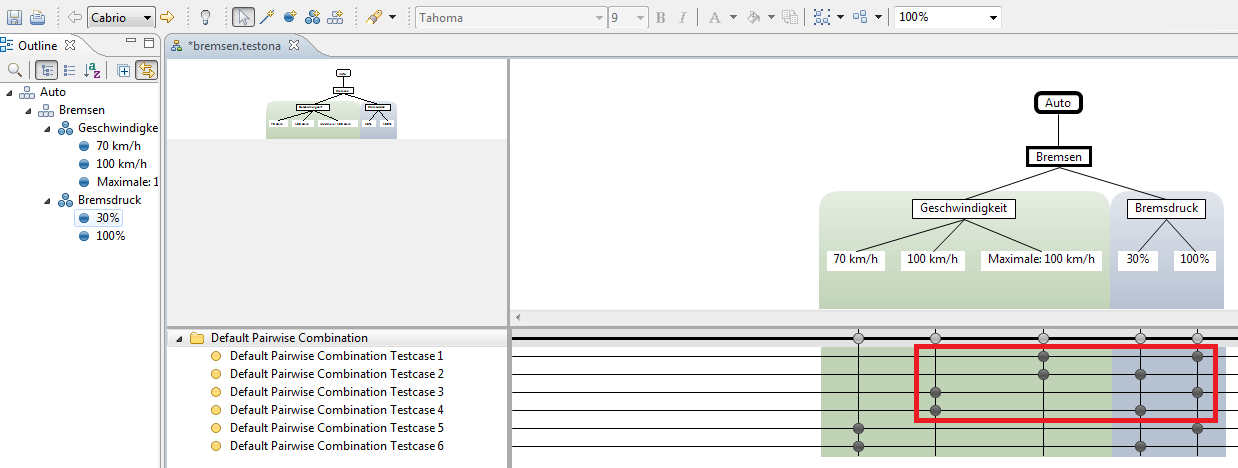
\includegraphics[scale=0.4]{4_3_cabrio.png}
  		  \caption{Aktive Variante Cabrio}
     \label{ttn.cases_cabrio}
  \end{center}
\end{figure}

\begin{figure}[h!]
  \begin{center}
    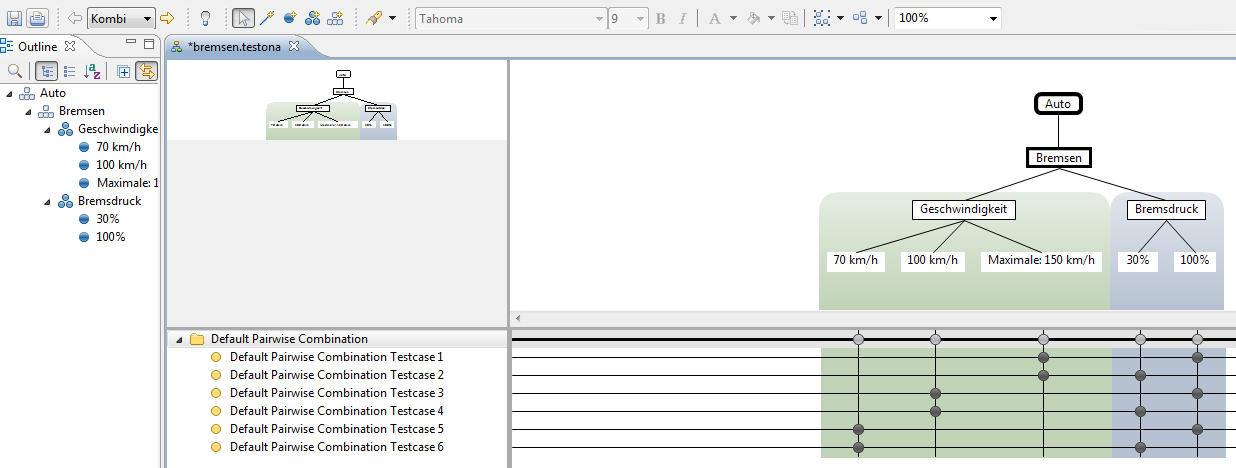
\includegraphics[scale=0.4]{4_3_kombi.png}
  		  \caption{Aktive Variante Kombi}
     \label{ttn.cases_kombi}
  \end{center}
\end{figure}

Es ist leicht zu erkennen, dass die Testfälle eins bis vier in der Variante \glqq Cabrio\grqq~ dupliziert sind. Bei einem minimalistischen Baum sind solche Fälle einfach zu erkennen. Bei einem komplexeren Baum mit sehr vielen Klassen kann es schnell zur Unübersichtlichkeit kommen. Duplizierte Testfälle könnten übersehen oder nicht erkannt werden.\\

Bei der Testfallgenerierung muss zusätzlich darauf geachtet werden (vorausgesetzt es gibt Varianten und Parameterwerte), dass nicht nur die Baumelemente sondern auch die Parameterwerte betrachtet werden.\\

Dafür müssen alle Klassen (Endknoten) unterhalb der gleichen Klassifikation überprüft werden. Nach dem obenstehenden Beispiel, müssen die Klassen \glqq 70 km/h\grqq , \glqq 100 km/h\grqq~ und \glqq Maximale\grqq~ verglichen werden. Da \glqq Maximale\grqq~ bei jeder Variante einen anderen Wert annimmt, muss hier überprüft werden, dass bei jeder Variante, sich der Wert nicht wiederholt. Die Werte werden aus dem geplanten \textit{ParameterTag} (siehe Abbildung \ref{ttn.objectGraph}) gelesen.

%#######################################################################################
%#######################################################################################
\newpage
\section{Benutzeroberfläche}
\paragraph{}

Eine Änderung der Benutzeroberfläche von TESTONA wurde mit Kollegen in der Entwicklung offen diskutiert. Als Ergebnis konnten wir aus Sicht der Entwickler feststellen, dass die bisherige Lösung als gut und intuitiv zu bezeichnen ist.\\

Um weitere Meinungen und Lösungsvorschläge zu sammeln habe ich Testingenieure die TESTONA mit Kunden anwenden in der Firma Berner \& Mattner befragt. Ein Ingenieur stellte fest, dass die Aktivierung der Variantenansicht unnötig ist. Er wünschte, dass die Variantenansicht als Hauptansicht definiert wird. 
Dass es einen Unterschied zwischen beiden Ansichten gibt liegt daran, dass verschiedene Etappen repräsentiert werden. Die Hauptansicht bietet verschiedene Features die in der Variantenansicht mit Variantenmanagement Features ergänzt werden. Dabei wird noch begründet, dass die Trennung zur Übersicht sehr viel beiträgt.\\

Als Ergebnis wurde festgelegt, dass für in dieser Arbeit gestellte Problemfrage nicht zur Unübersichtlichkeit der Benutzeroberfläche beiträgt. Es wird erhofft, dass außer der Erweiterung der Funktionalität, dass auch die Übersicht verbessert wird. Die Trennung zwischen der Hauptansicht und der Variantenansicht wird beibehalten ebenso die Lösung der Pfeile und des Drop-Down Menüs (siebe Abbildungen \ref{ttn.generic}, \ref{ttn.2}, \ref{ttn.3}).
